\section{Leaderboard}

En Kaggle me di de alta como LuisUGR, ya que en la primera clase en la que se explicó el guión se dijo que usaramos: -DNI o -UGR. Dias después, intenté cambiarlo pero siempre salía que se había cambiado con éxito, pero realmente no se aplicaba.

\begin{figure}[H]
\centering
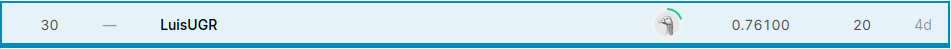
\includegraphics[width=\textwidth]{imagenes/leaderboard.png}
\caption{Fila de la competición correspondiente}
\end{figure}

\section{Predicción de precios de coches usados}

\subsection{Descripción del problema}

Tenemos un conjunto de datos de vehículos usados, clasificados estos en 5 categorías: del 1 al 5 dependiendo del precio(desde los más baratos a más caros, respectivamente). Debemos de poder predecir la categoría a la que pertenece un coche(clasificación multiclase).

\begin{figure}[H]

\begin{subfigure}{.5\textwidth}
  \centering
  \includegraphics[width=0.8\textwidth]{imagenes/features/Año.png}
  \caption{Año}
\end{subfigure}%
\begin{subfigure}{.5\textwidth}
  \centering
  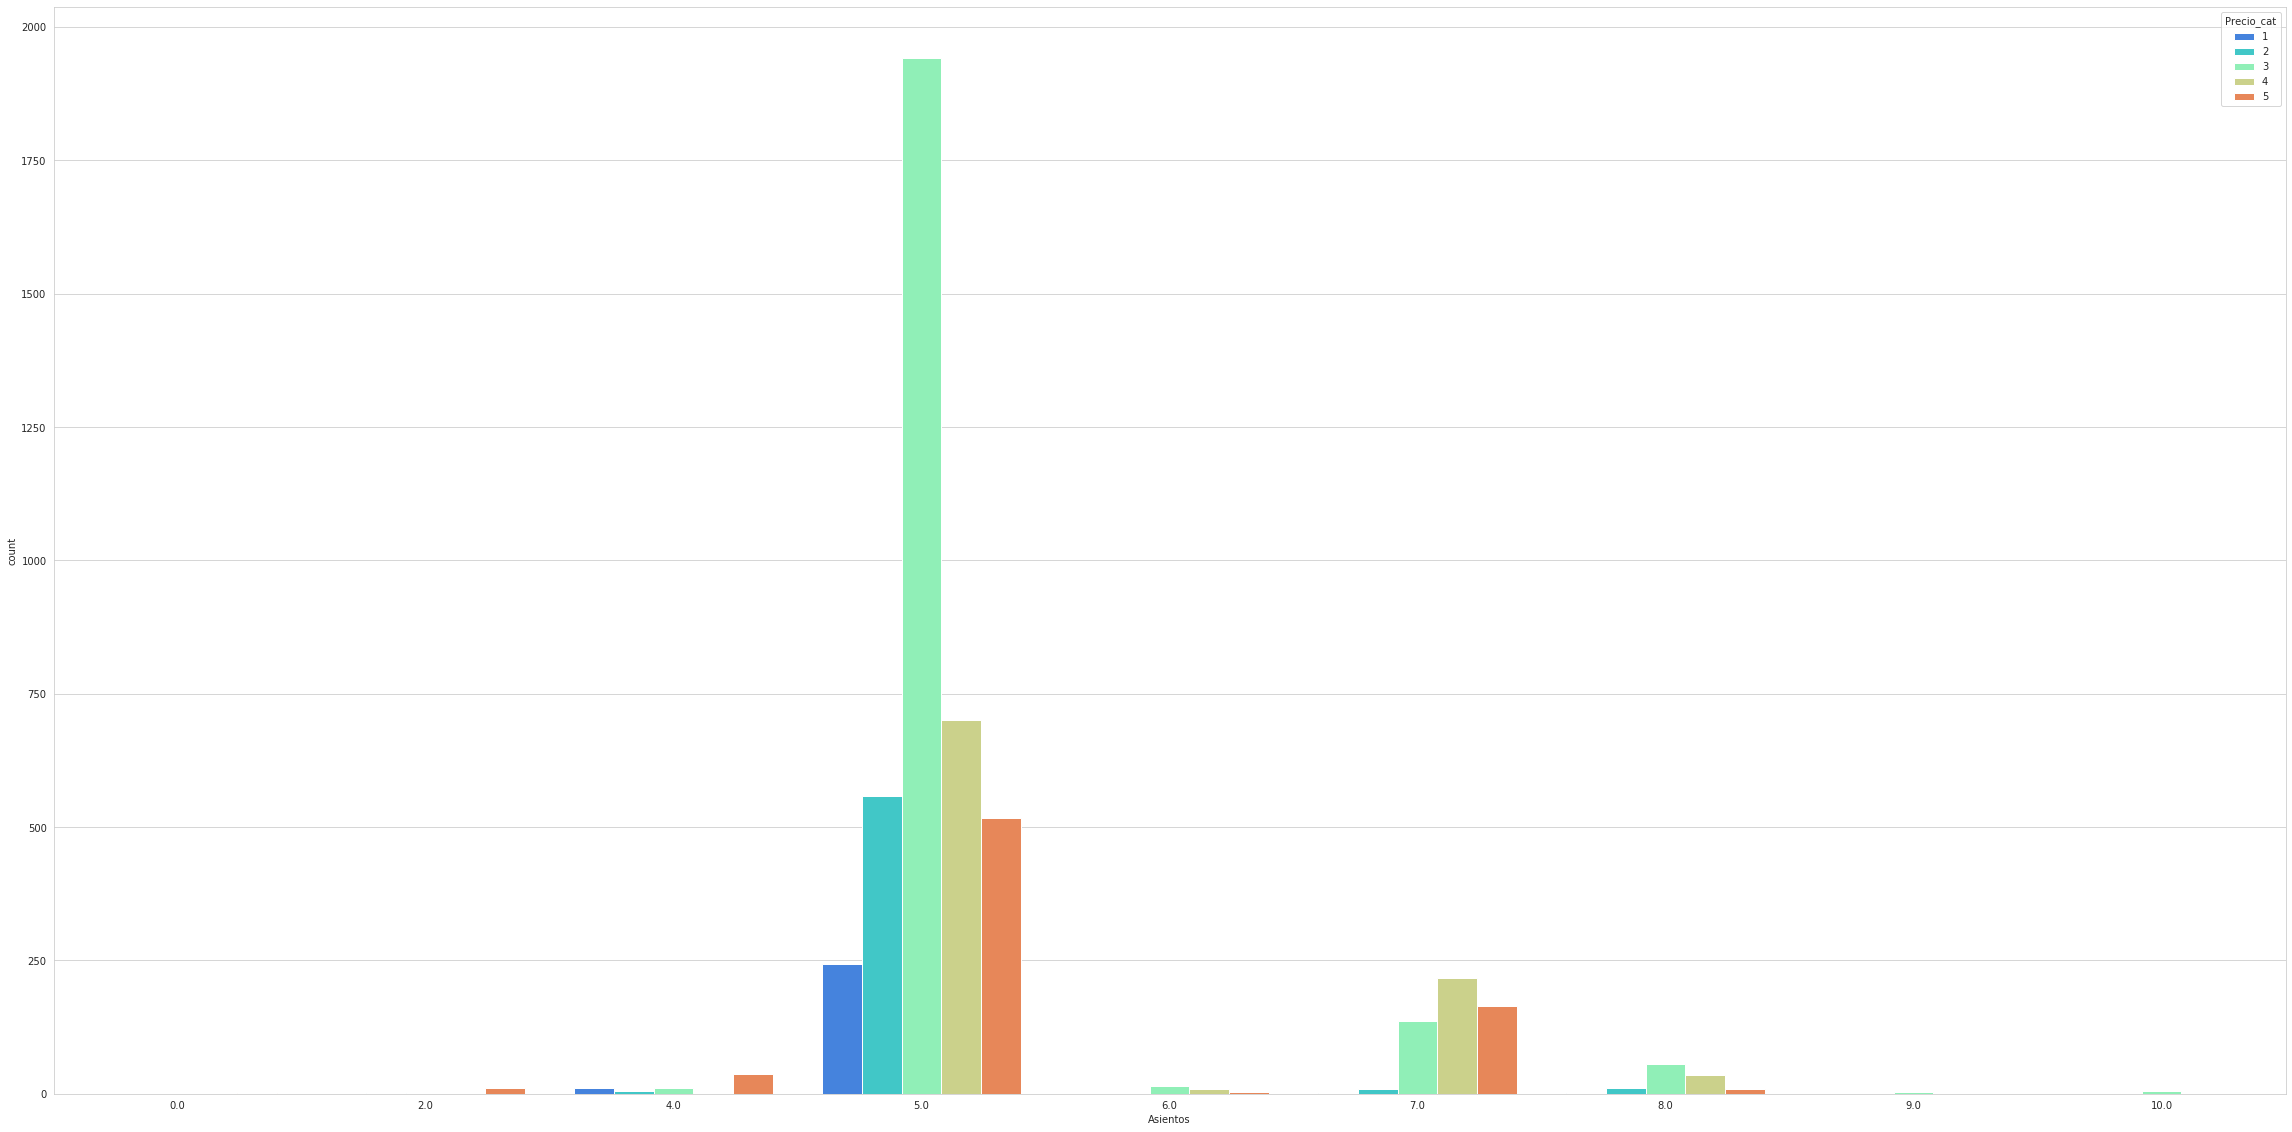
\includegraphics[width=0.8\textwidth]{imagenes/features/Asientos.png}
  \caption{Asientos}
\end{subfigure}
\begin{subfigure}{.5\textwidth}
  \centering
  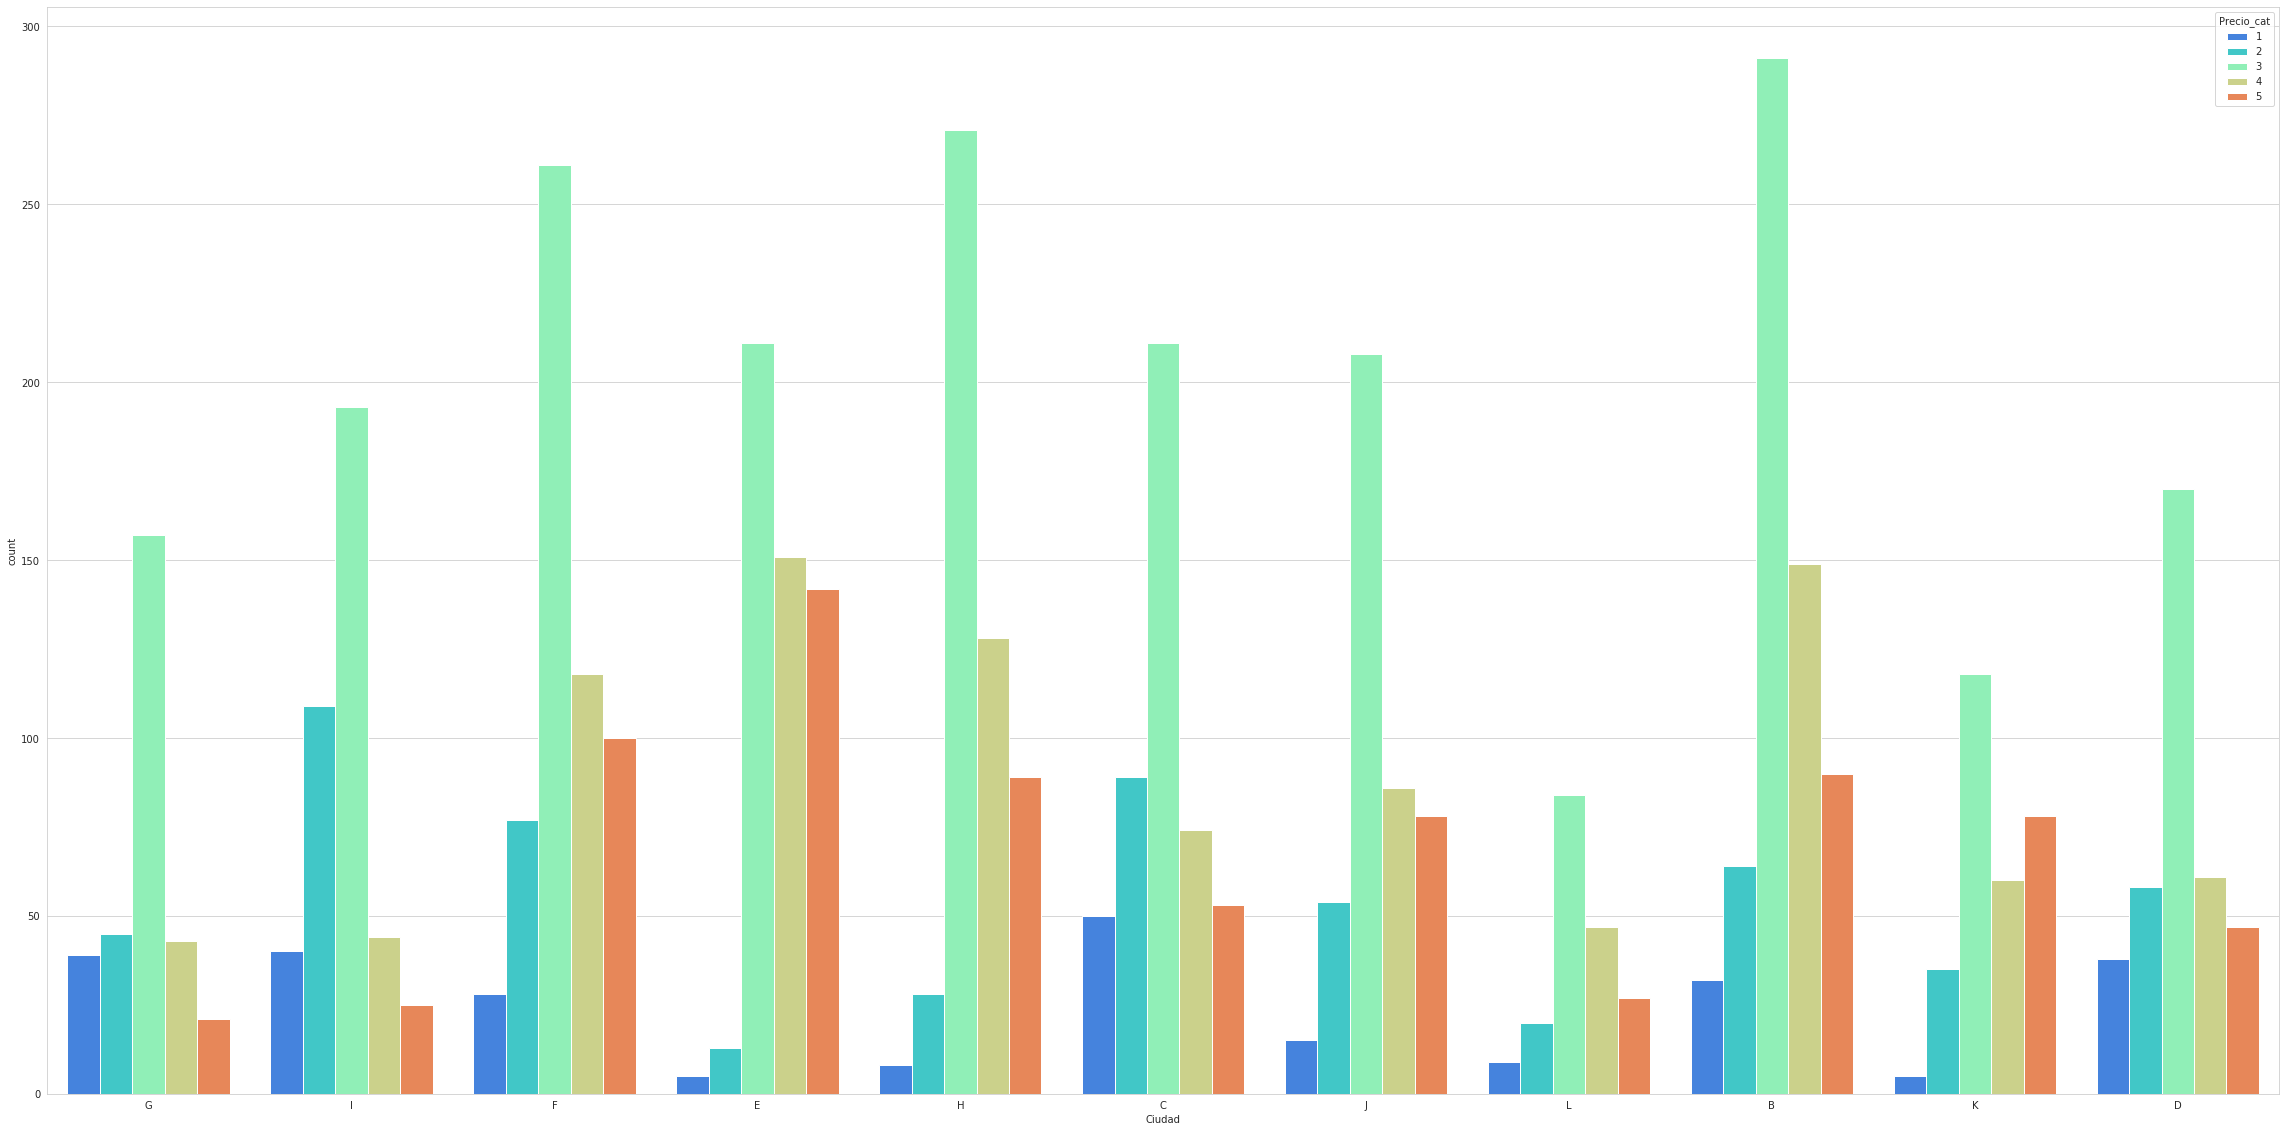
\includegraphics[width=0.8\textwidth]{imagenes/features/Ciudad.png}
  \caption{Ciudad}
\end{subfigure}%
\begin{subfigure}{.5\textwidth}
  \centering
  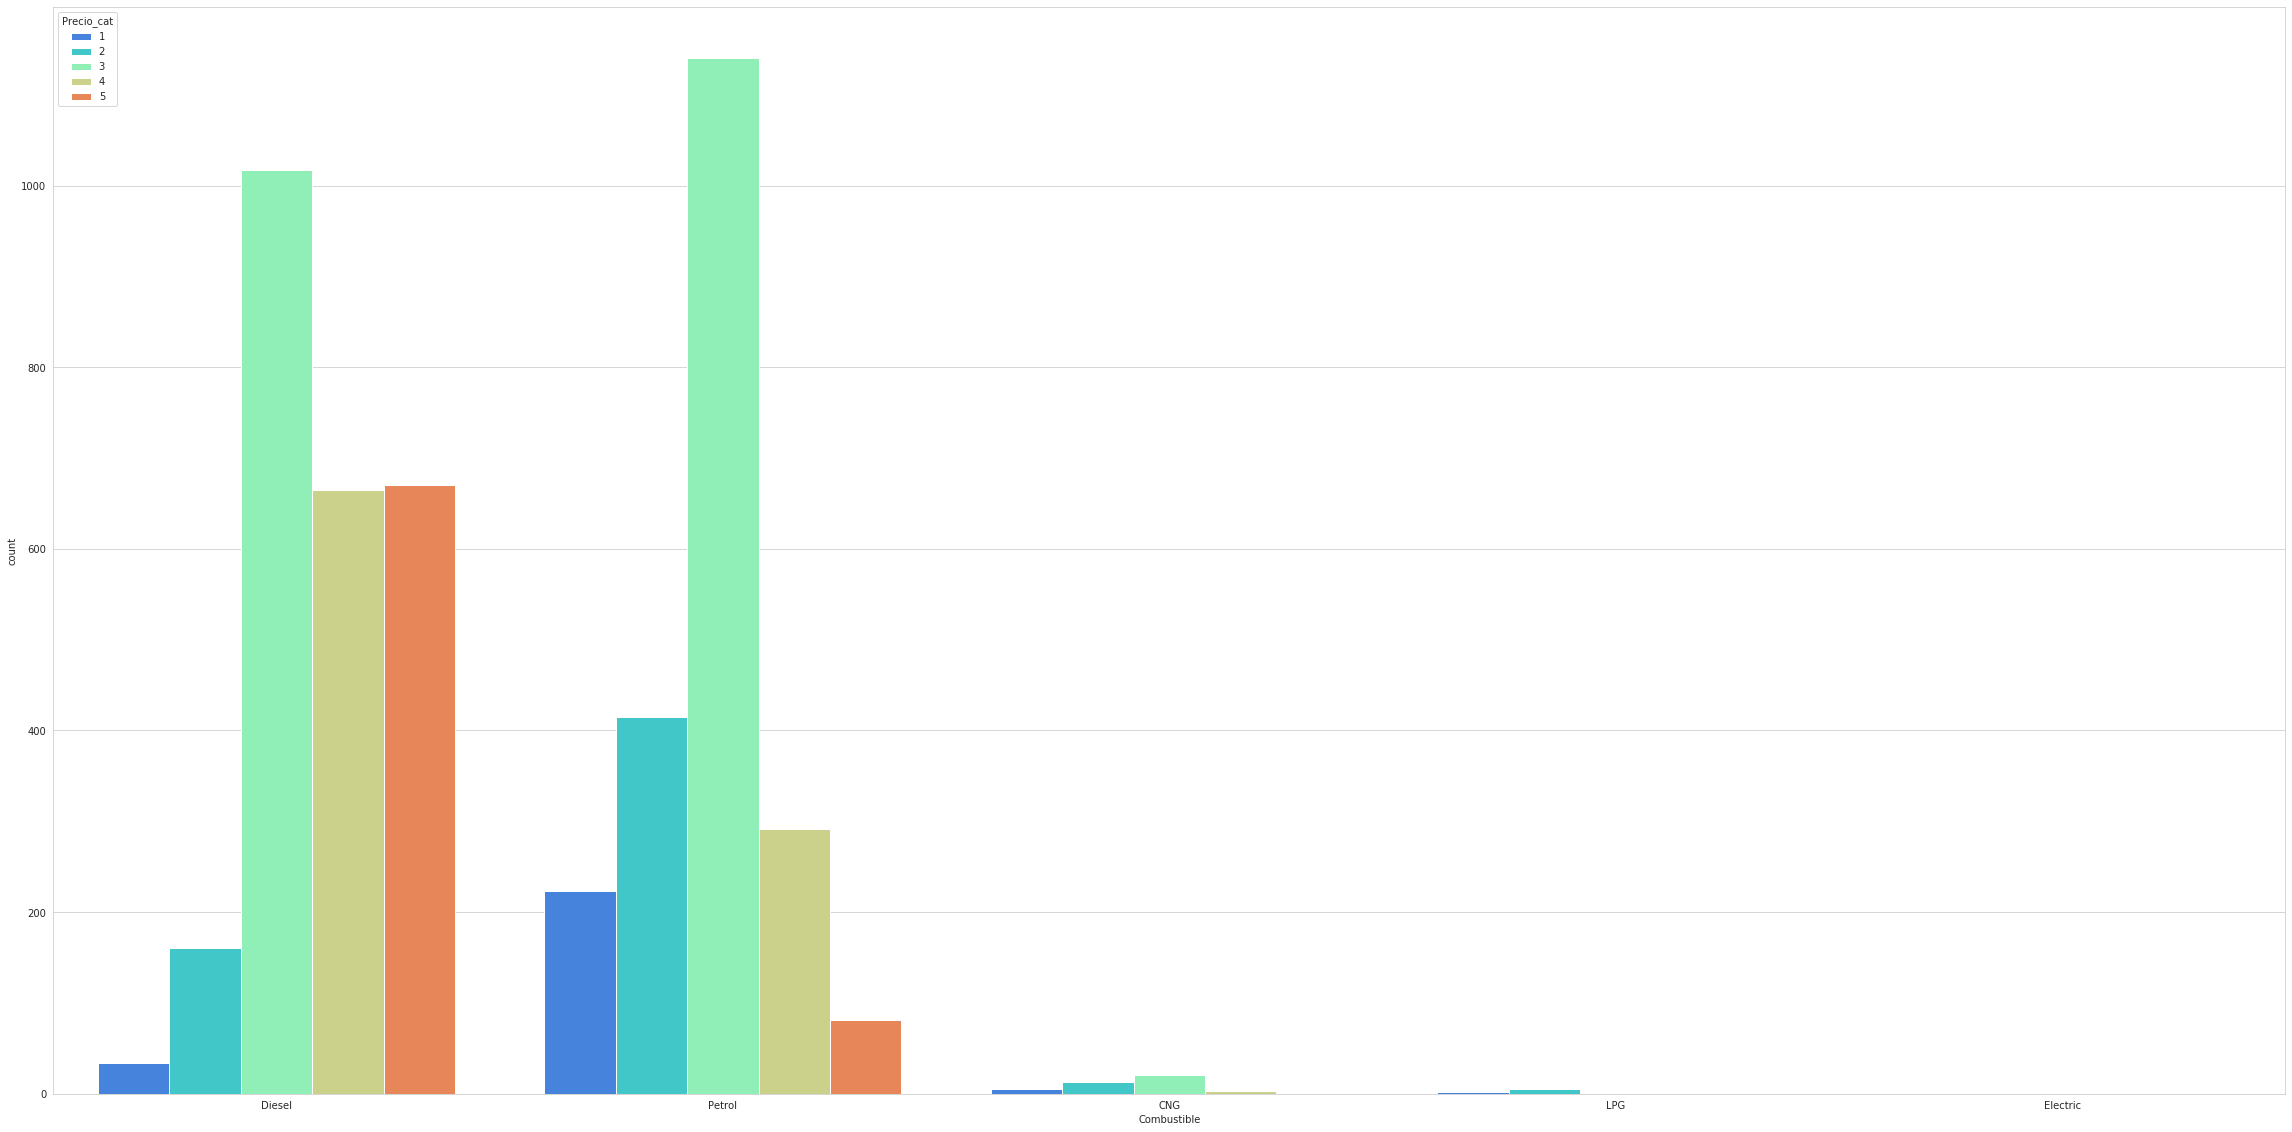
\includegraphics[width=0.8\textwidth]{imagenes/features/Combustible.png}
  \caption{Combustible}
\end{subfigure}
\begin{subfigure}{.5\textwidth}
  \centering
  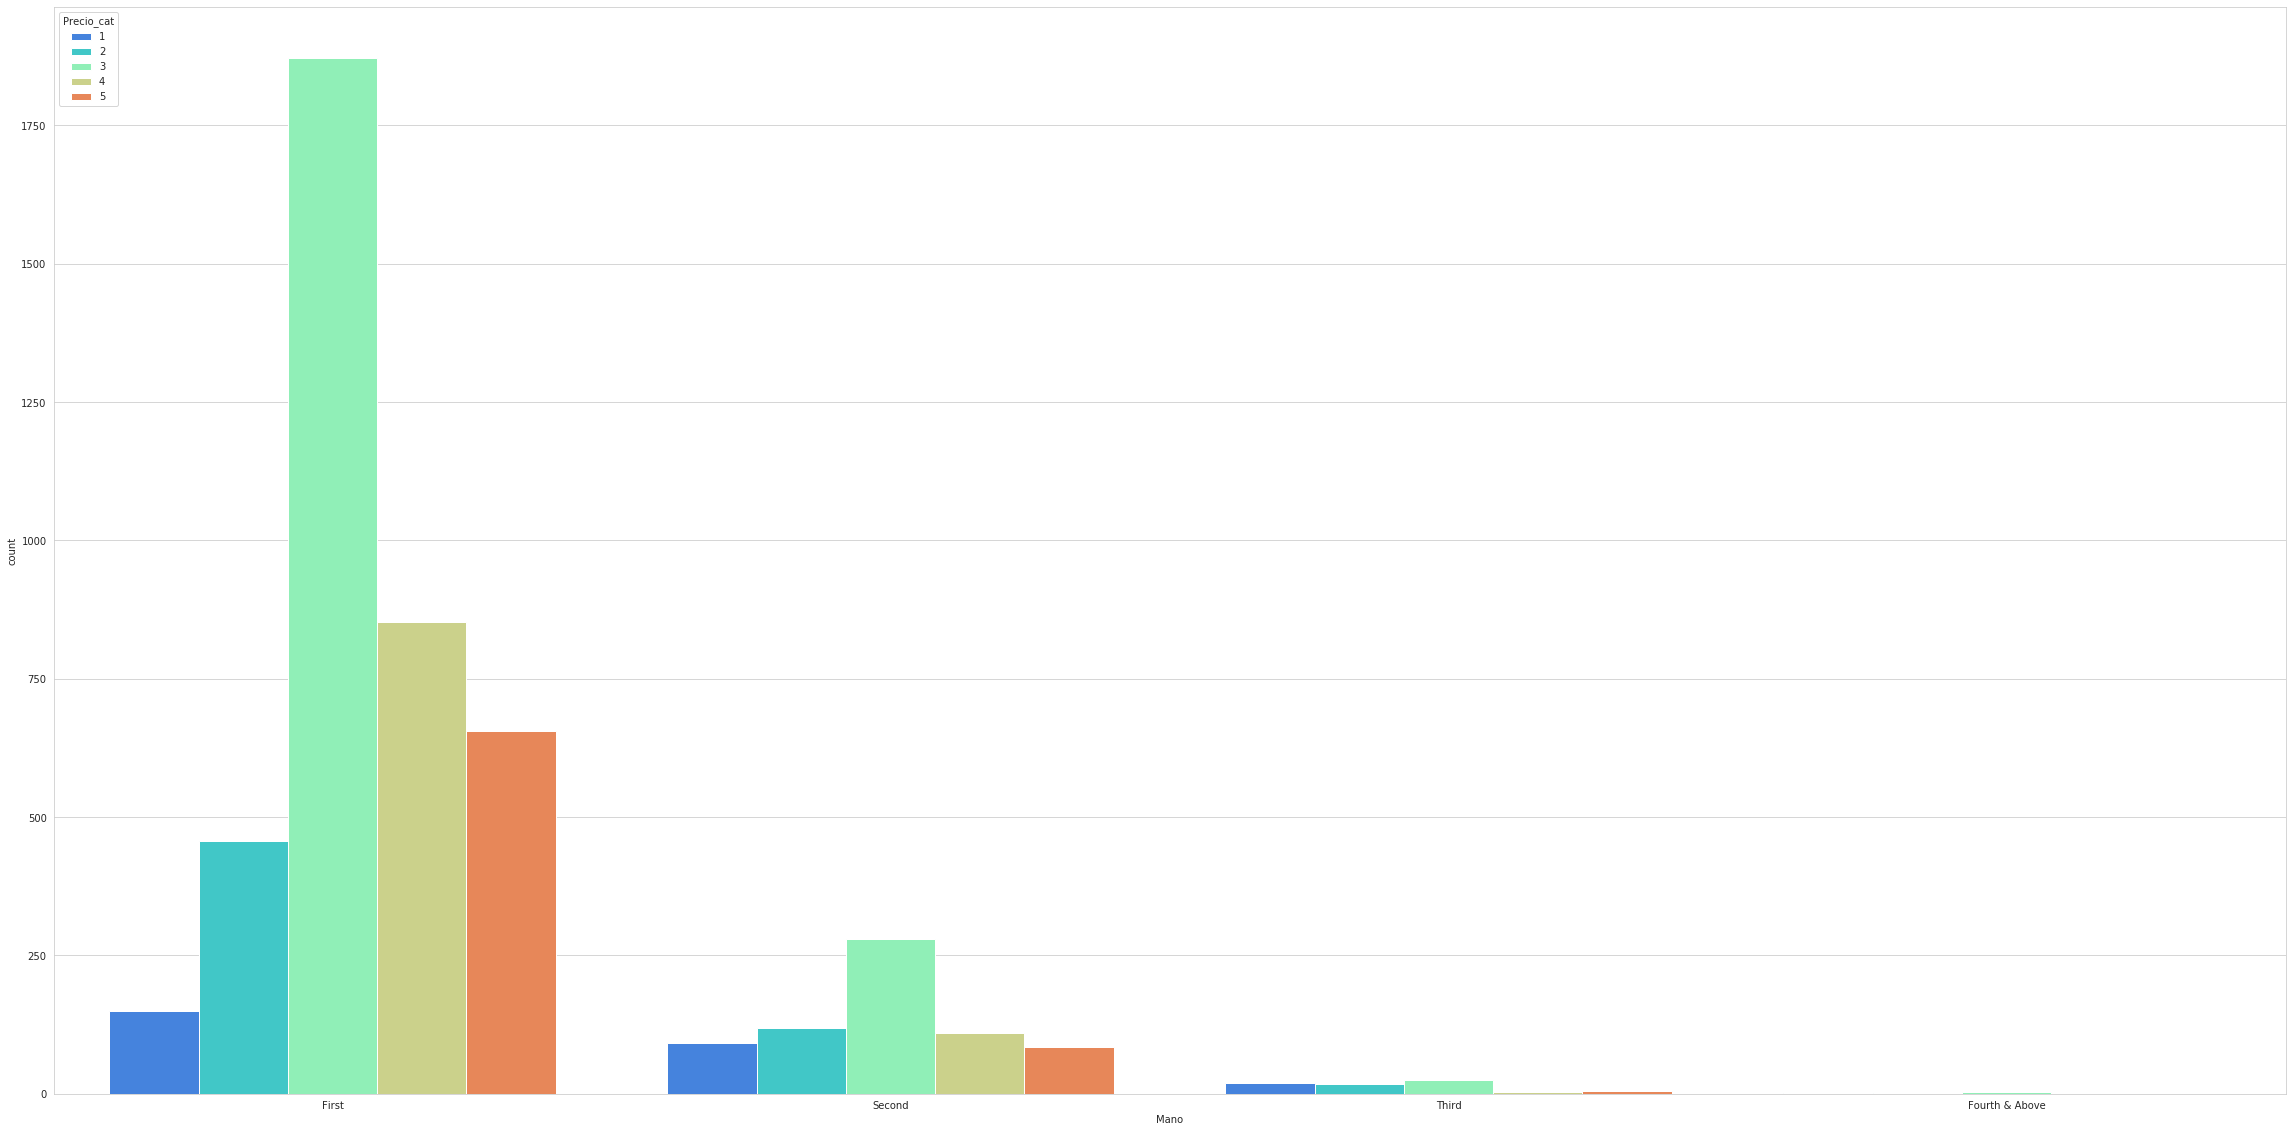
\includegraphics[width=0.8\textwidth]{imagenes/features/Mano.png}
  \caption{Mano}
\end{subfigure}%
\begin{subfigure}{.5\textwidth}
  \centering
  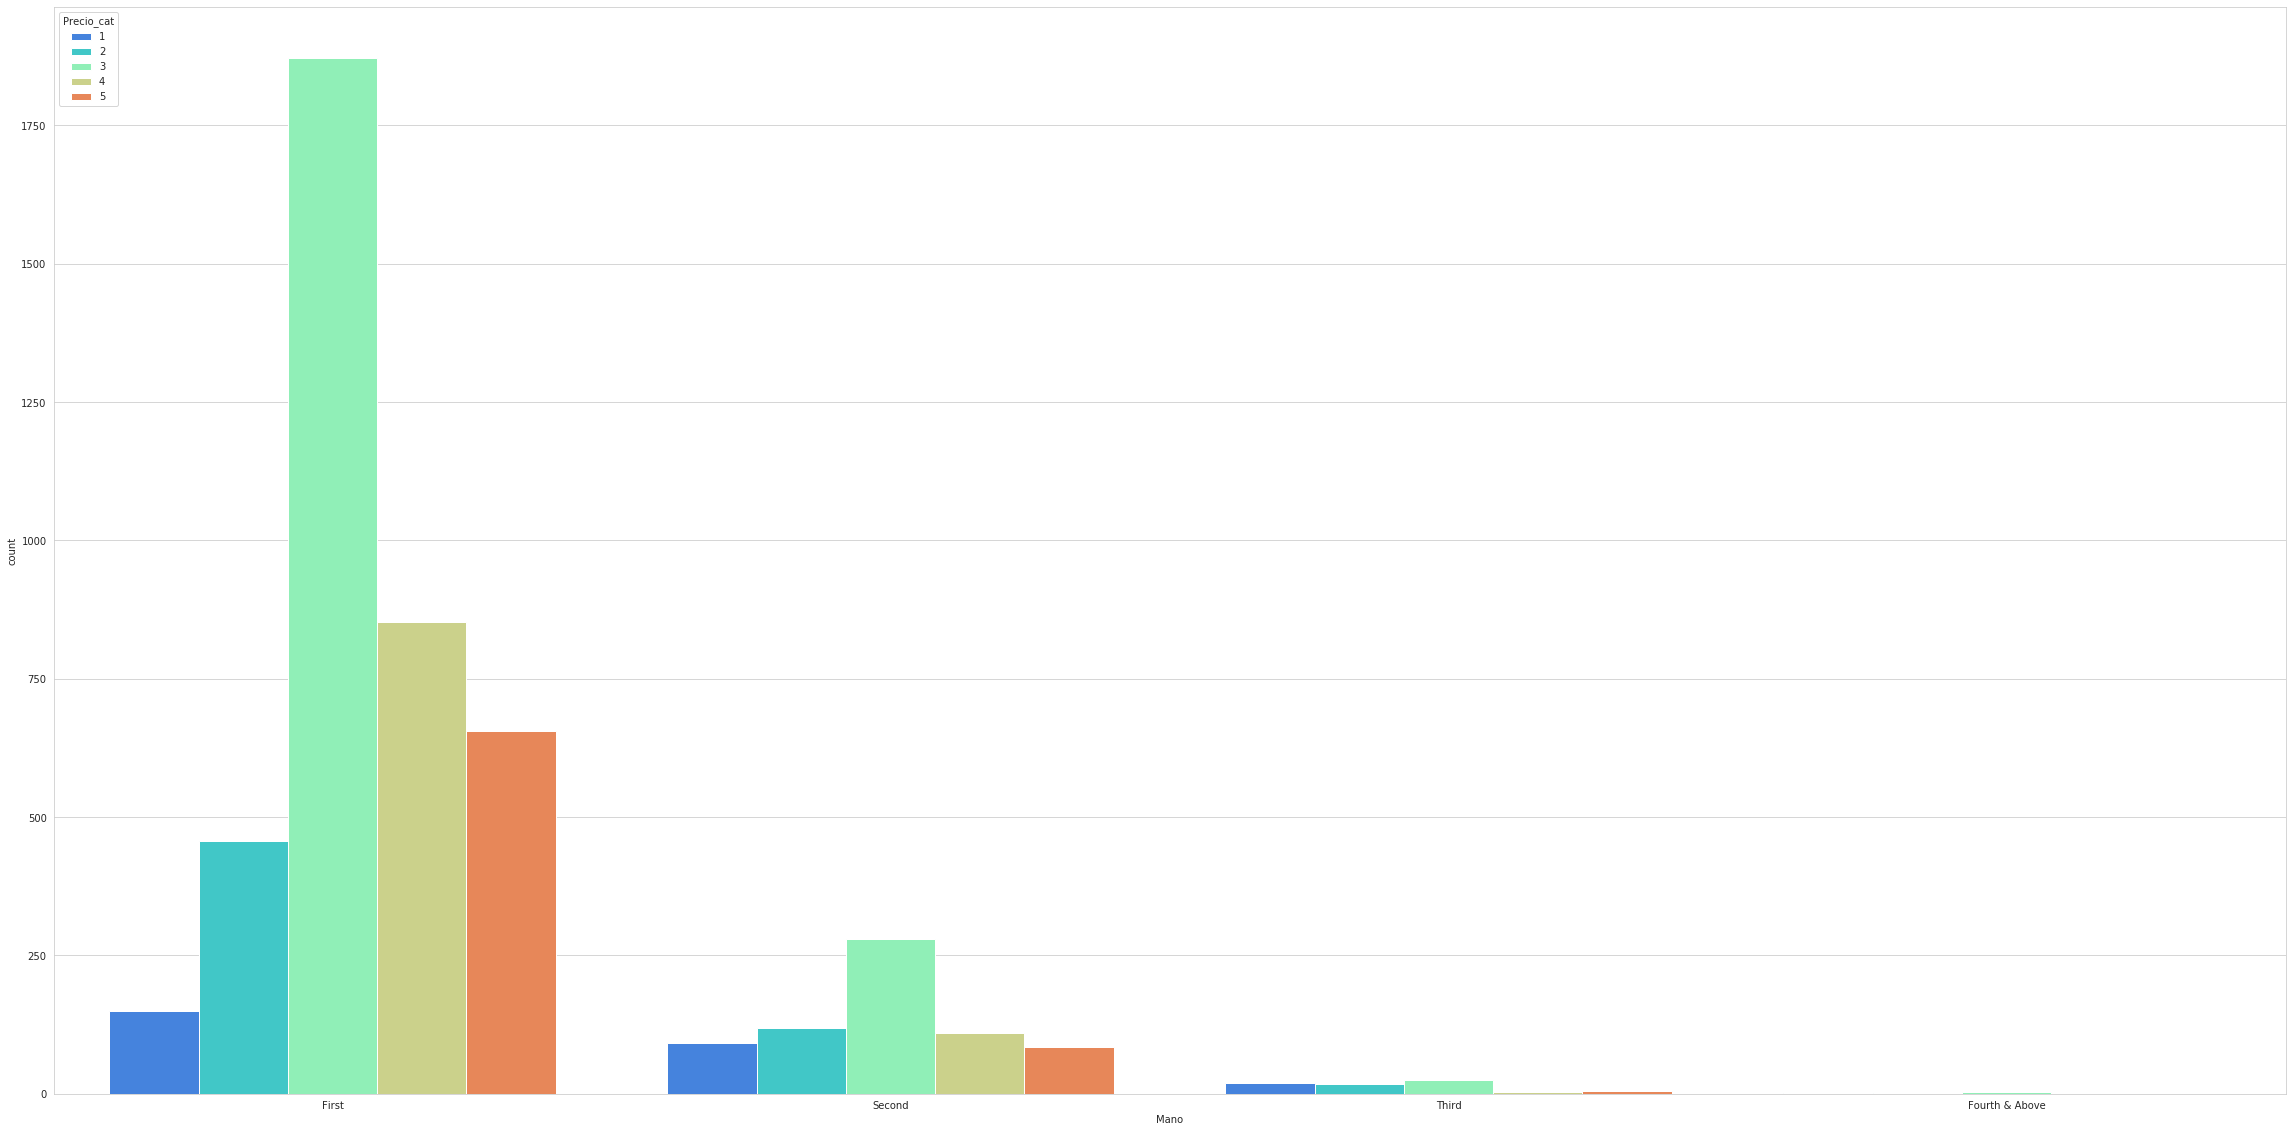
\includegraphics[width=0.8\textwidth]{imagenes/features/Mano.png}
  \caption{Mano}
\end{subfigure}
\begin{subfigure}{.5\textwidth}
  \centering
  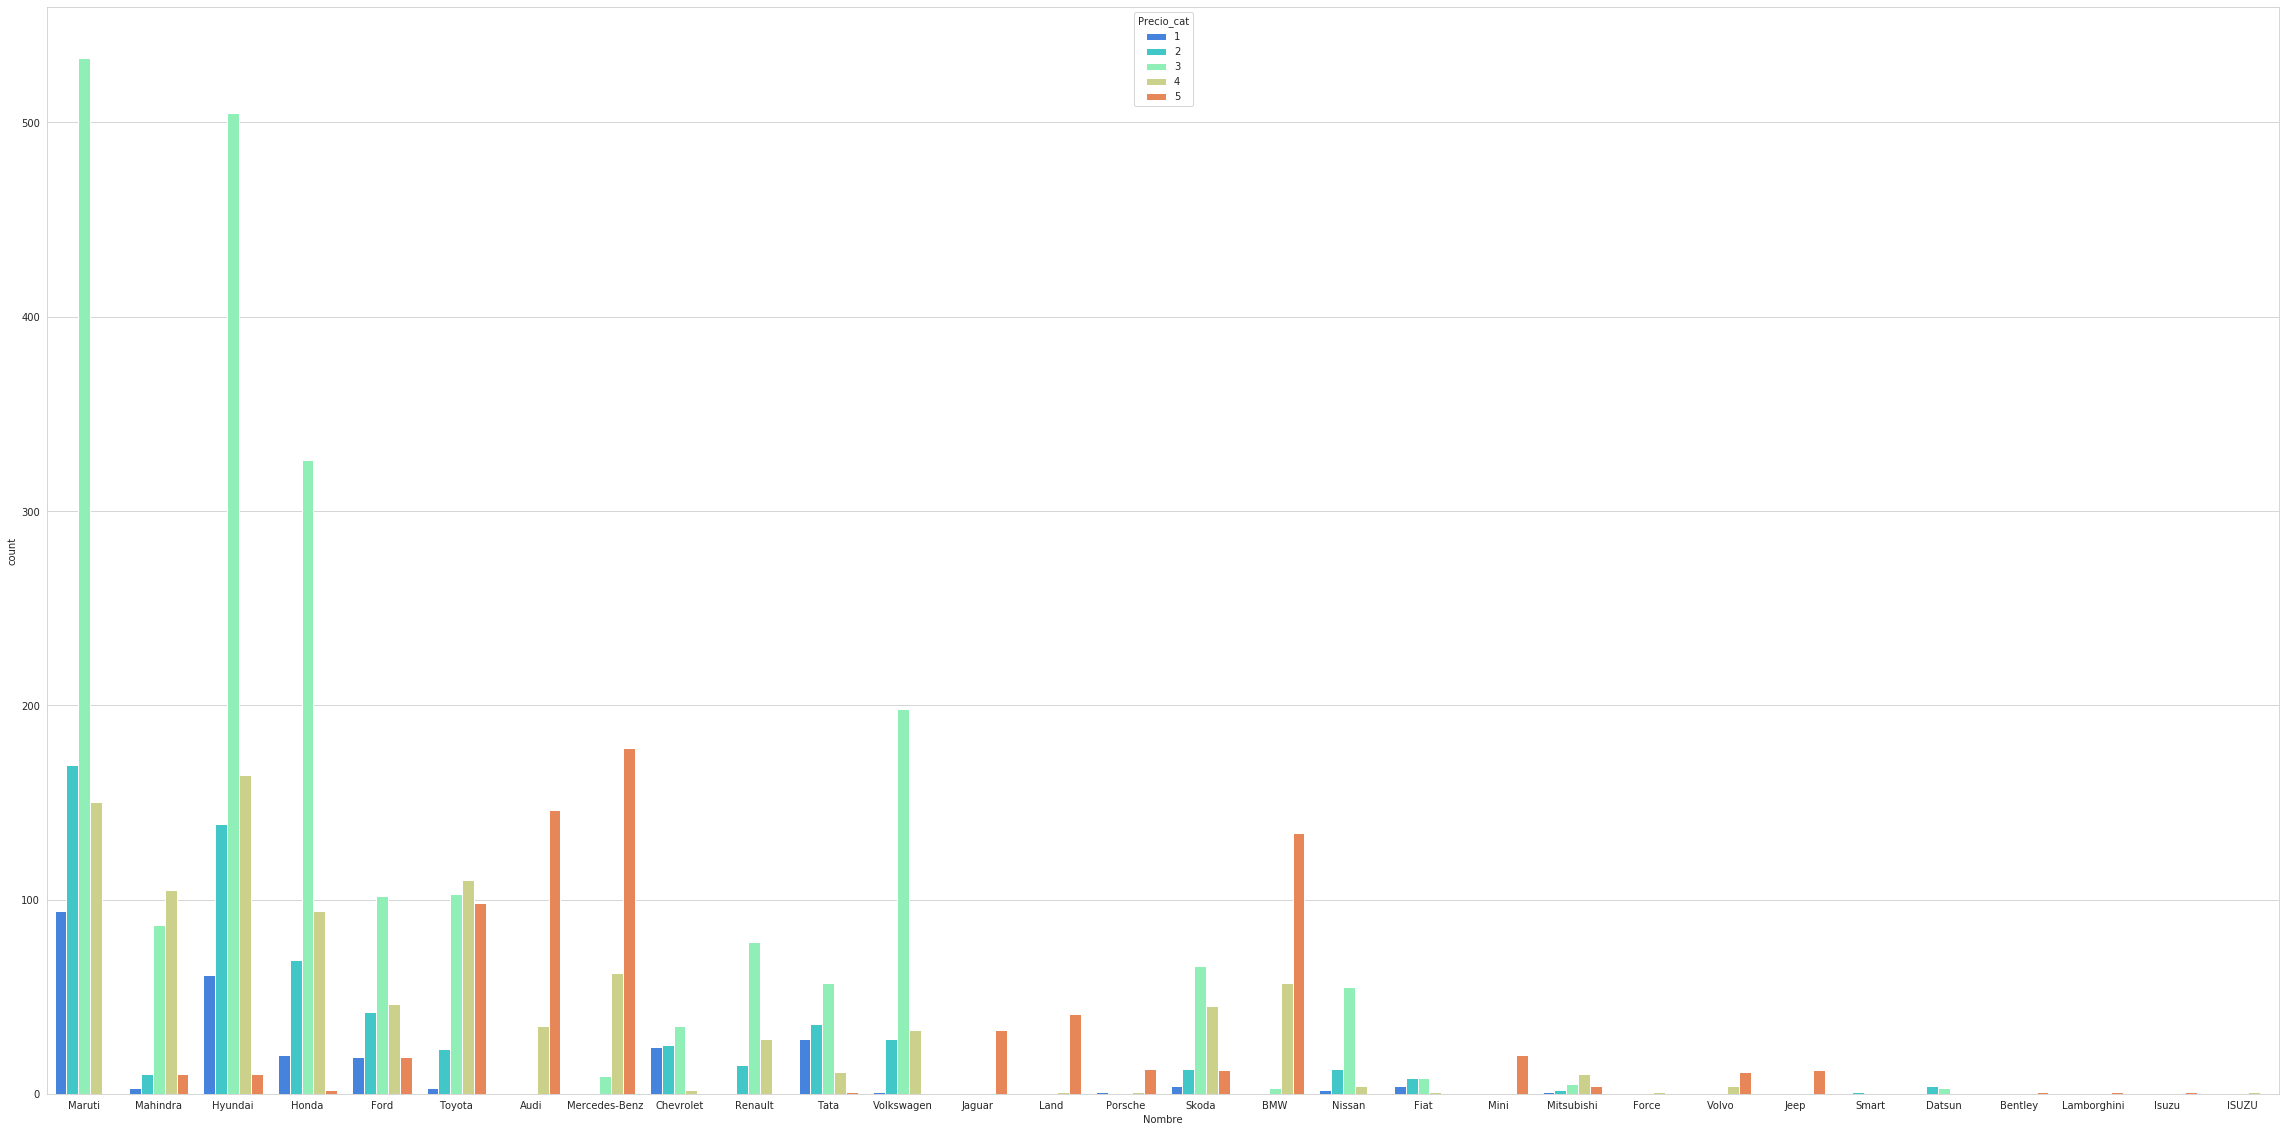
\includegraphics[width=0.8\textwidth]{imagenes/features/Nombre.png}
  \caption{Marca del vehículo}
\end{subfigure}%
\begin{subfigure}{.5\textwidth}
  \centering
  \includegraphics[width=0.8\textwidth]{imagenes/features/Tipo_Marchas.png}
  \caption{Tipo de marchas}
\end{subfigure}

\caption{Presencia de cada variable en las distintas clases representadas en Precio\_cat}
\label{fig:fig}
\end{figure}

\begin{figure}[H]
\centering
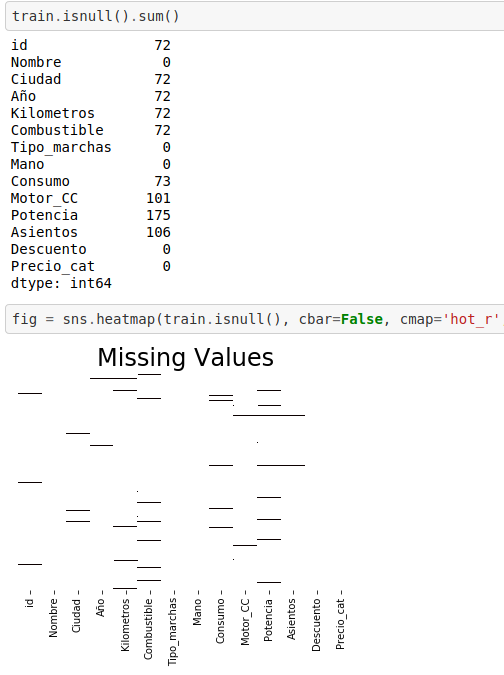
\includegraphics[width=0.8\textwidth]{imagenes/mv.png}
\caption{Valores perdidos en el dataset de entrenamiento.}
\end{figure}

\begin{figure}[H]
\centering
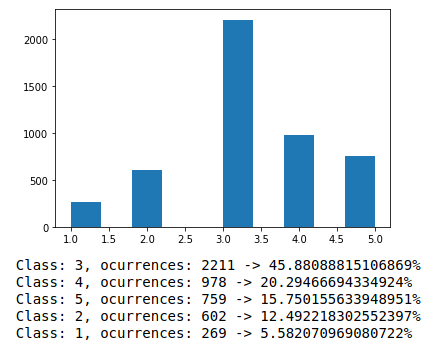
\includegraphics[width=0.8\textwidth]{imagenes/classes.png}
\caption{Ocurrencias de las clases}
\end{figure}

Como bien sabíamos, se trata de un problema con múltiples clases y en este caso, desbalanceadas.
